\begin{post}
	\postdata{Between the South and the North}{2011}{11}{05}{01}{02}{37}
	\begin{content}
I did it. I went there. North Korea, officially the Democratic People's Republic of Korea, the evil twin of South Korea, the loser clenched in between the two Asian superpowers. Today, I, for the first time, stepped on the North Korean territory. The story behind it is not special, so I apologize to those of you who expected something from a lame action movie with explosions, car chases, spy gadgets and hot girls.

\begin{wrapfigure}{r}{0.45\textwidth}
\vspace{-12pt}
\centering\fbox{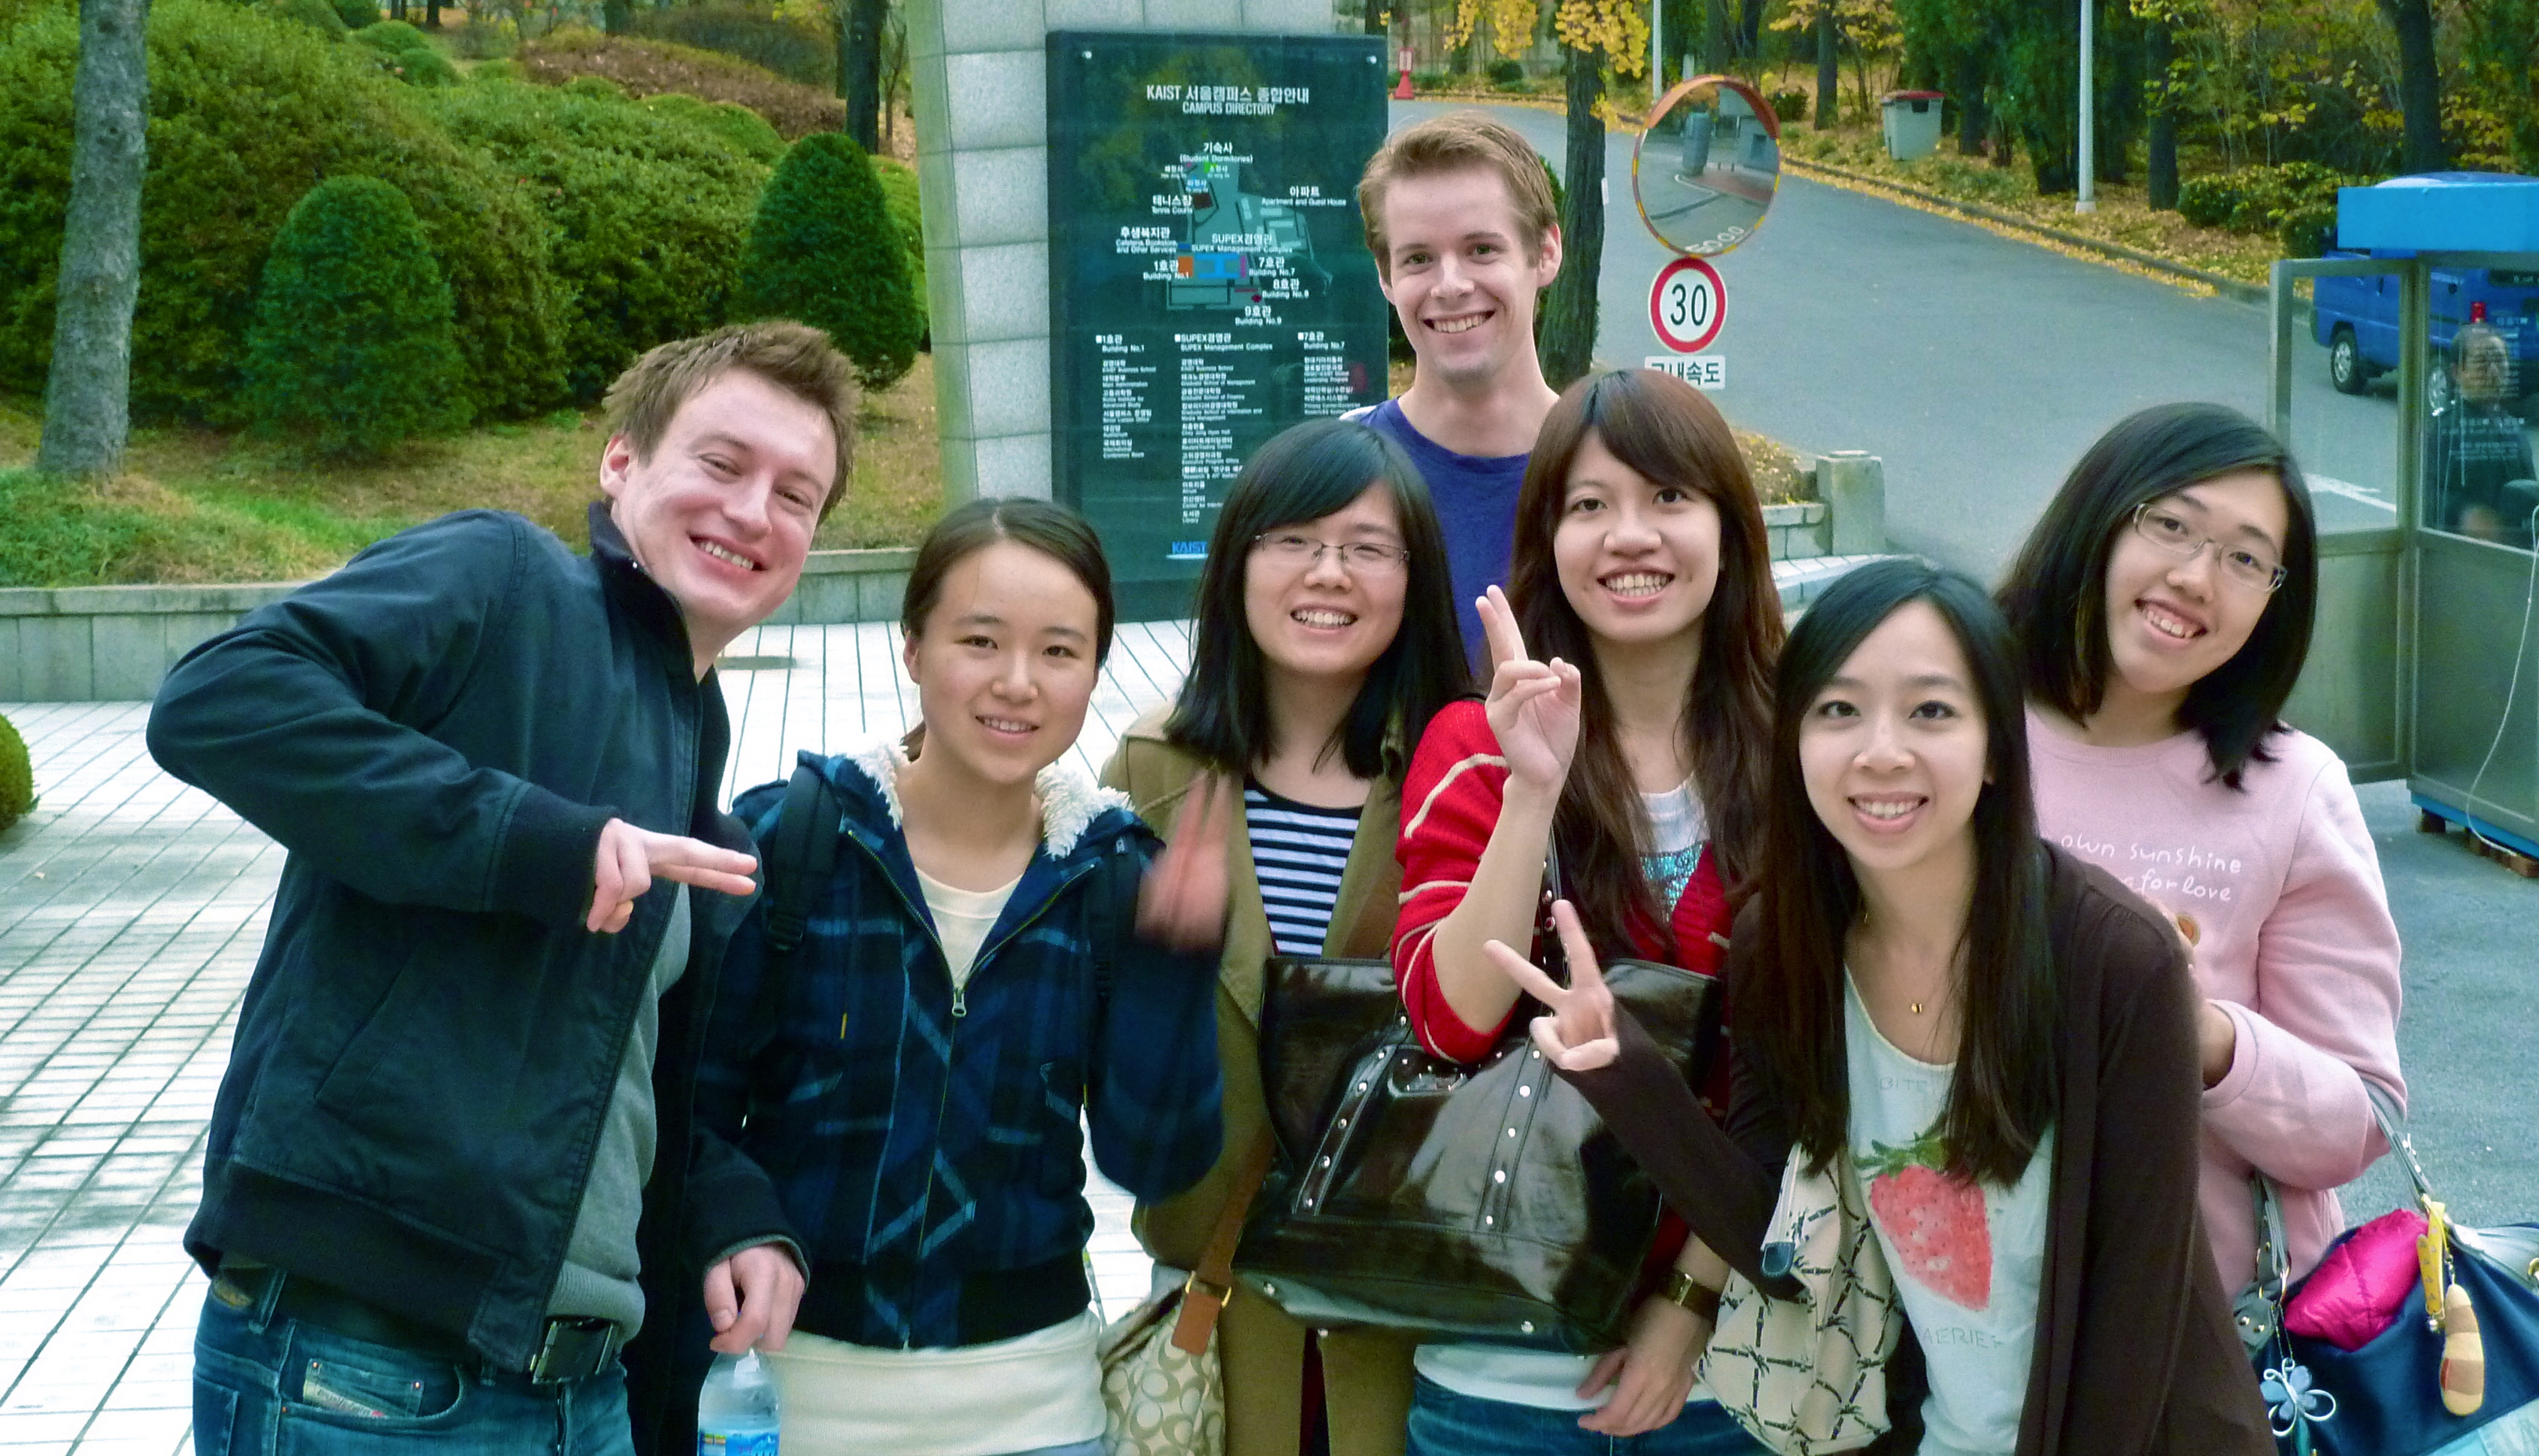
\includegraphics[width=0.45\textwidth]{photos/11/05/p1010277.jpg}}
\end{wrapfigure}As we planned earlier, today we went on the "DMZ trip", i.e. trip to the demilitarized zone, which lies between North and South Korea. Despite it's name, DMZ is the most militarized border in the world, with permanent military presence on both sides, and it stretches across the whole Korean peninsula in a 4km wide corridor. For a regular mortal it is merely impossible to cross the border, because DPRK does not allow anyone from the South Korean side to cross the border. However, the DMZ, and the associated Joint Security Area (JSA) are partially opened for public through numerous agencies offering tour packages.

Our bus picked us up at the campus at 7:10am. Waking up so early was extremely painful, especially due to previous night at Indy Pub. My efforts to sleep in the bus were hampered by my slightly nauseous state, which fortunately got better 30 minutes into the trip. After picking up the rest of our tour group at Lotte Hotel, we set off for the DMZ, which is about 1hr drive from Seoul.

\begin{wrapfigure}{r}{0.3\textwidth}
\centering\fbox{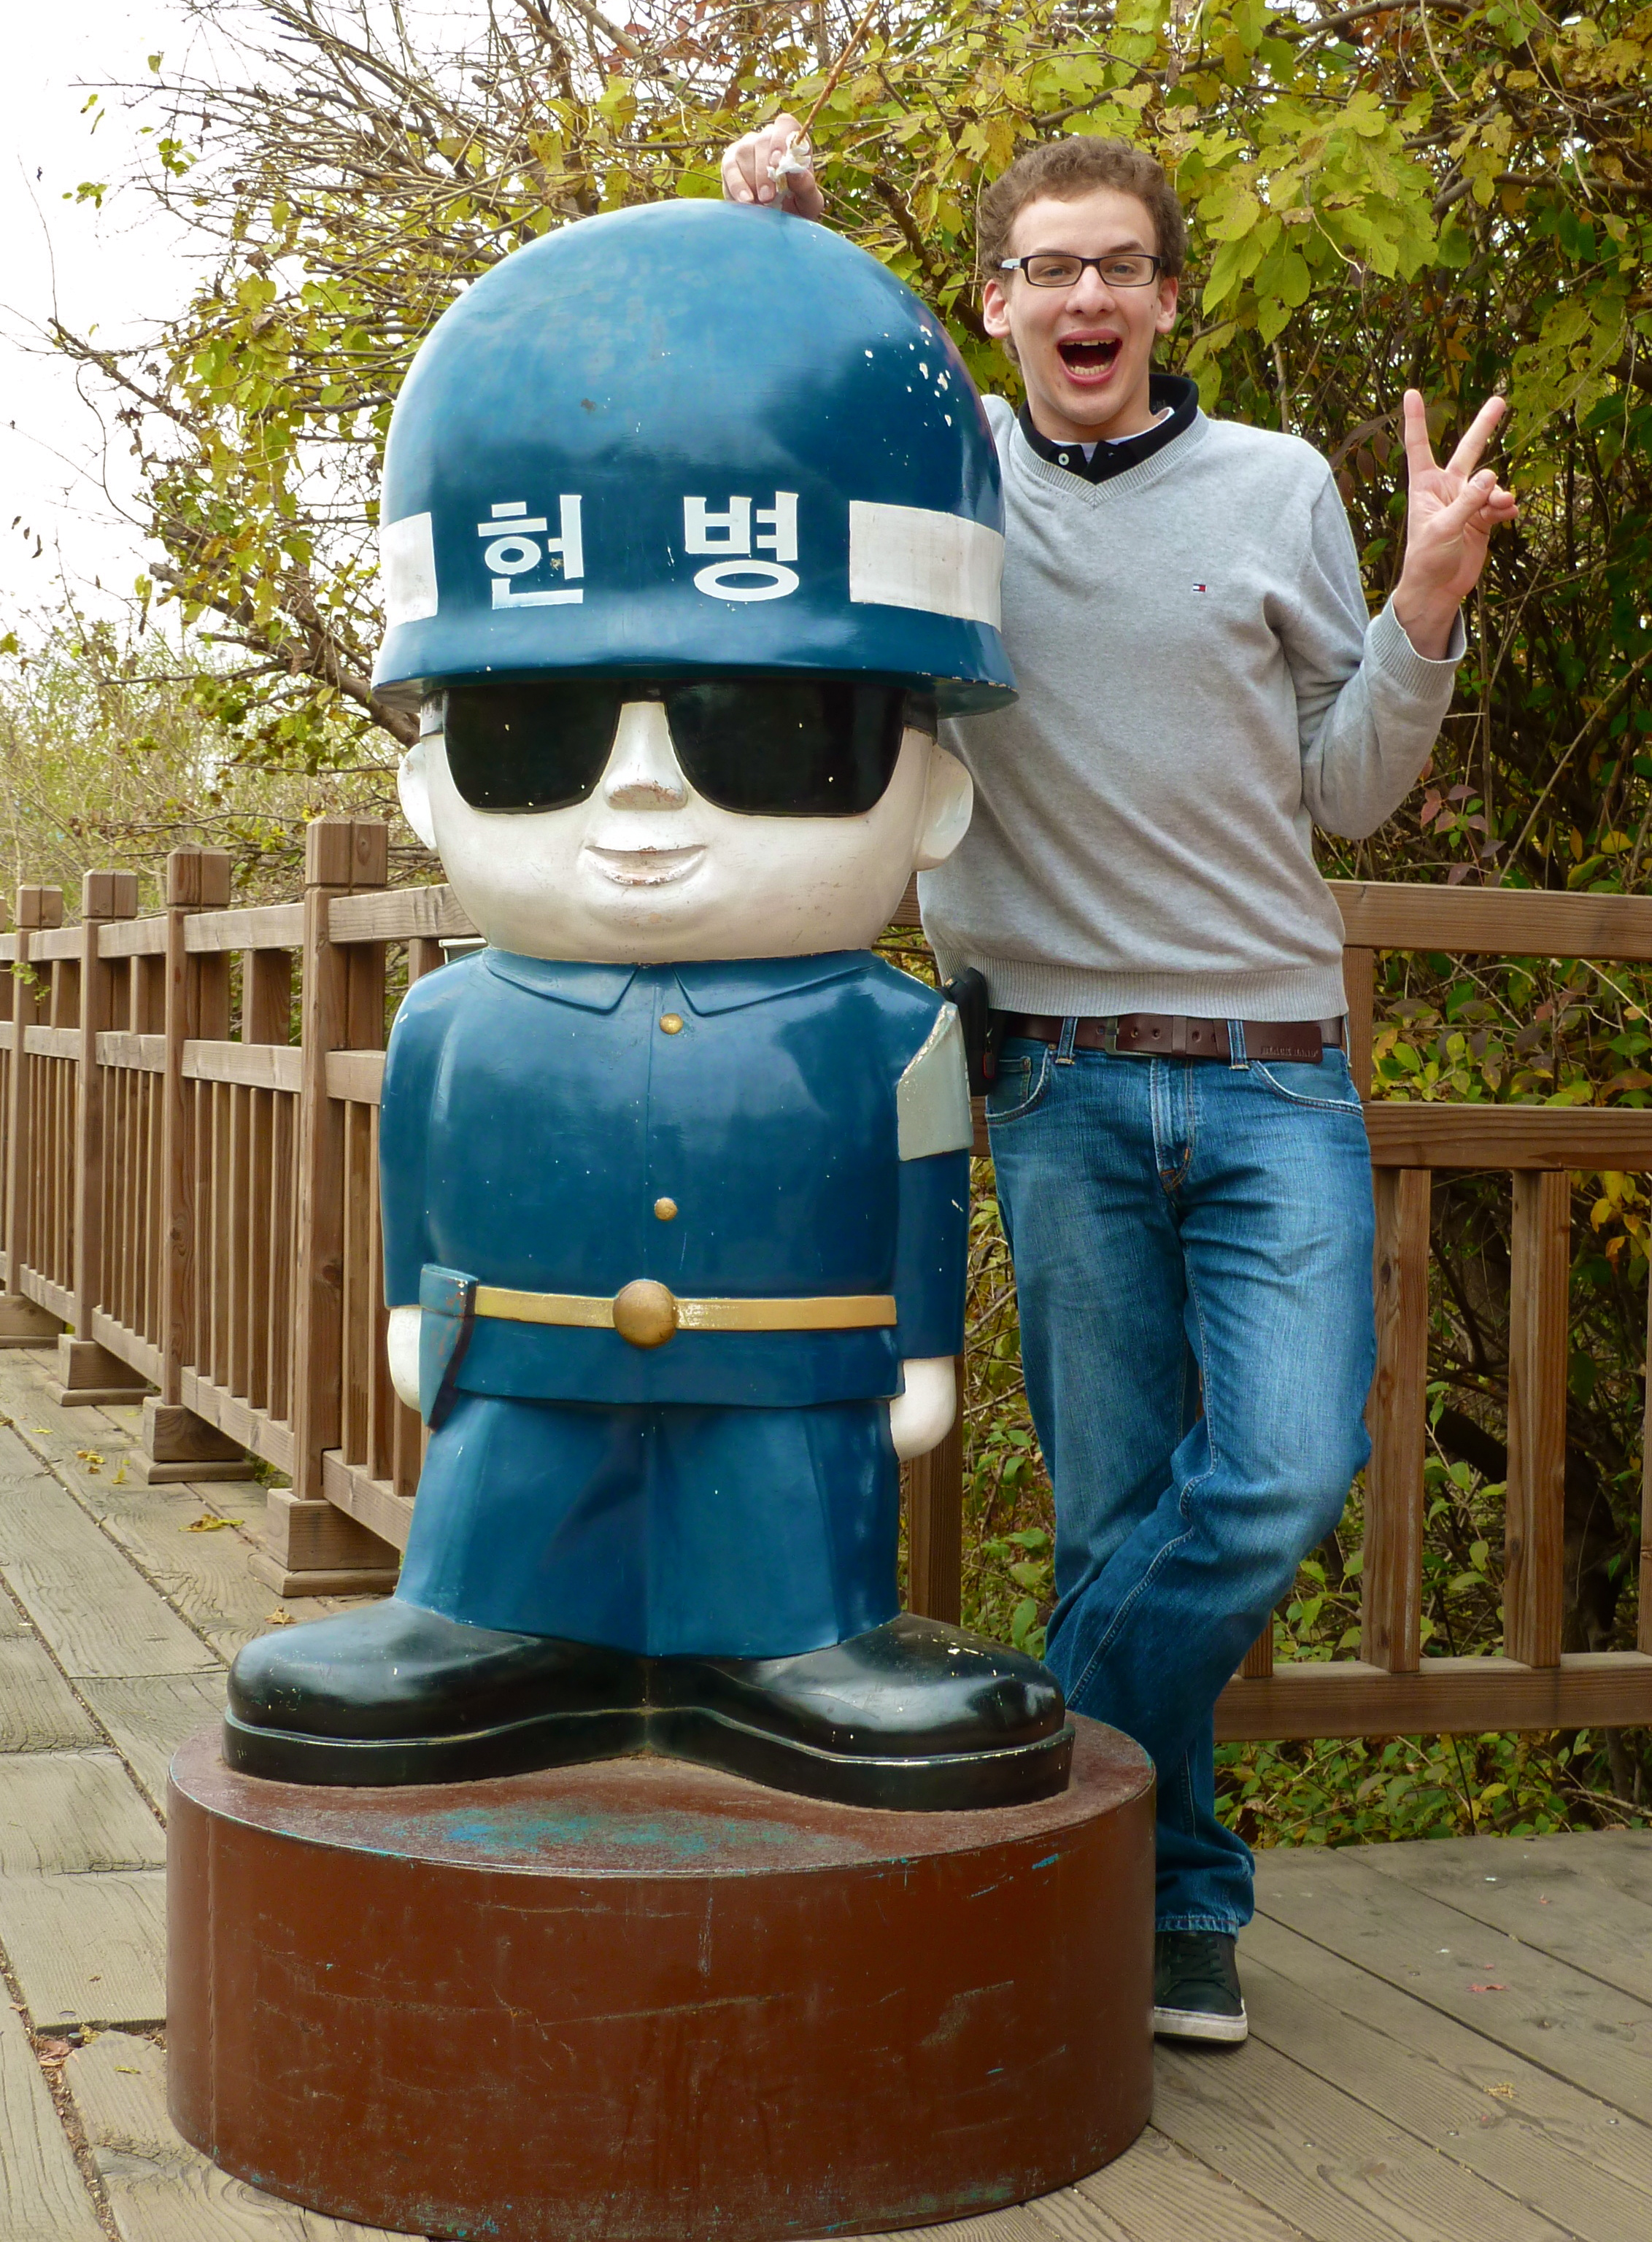
\includegraphics[width=0.3\textwidth]{photos/11/05/p1010280.jpg}}
\vspace{-26pt}
\end{wrapfigure}Our first stop was at the Freedom bridge, which was used as a place for trading prisoners of war after the Korean War in 1950s. As a first stop, it was not that interesting because it was simply a bridge. At least we got some breakfast, though:)

The second stop was the 3rd infiltration tunnel, also called the Third Tunnel of Aggression. It is one of the tunnels that North Koreans were planning to use for their invasion to South Korea. So far, there have been 4 tunnels revealed, however, rumors say that there are many more unfinished. The fun fact about this tunnel is that in order to explain the existence of such tunnel during a cease fire time, North Koreans painted the walls of this tunnel black and claimed they were mining coal. The tunnel is still "open", i.e. it would theoretically be possible to go to the other side, however, there are 3 concrete barricades to avoid access from NK. The tunnel is 73m underground and access for tourists is realized by a very steep 300m shaft. The tunnel ceiling is quite low, which means you have to walk bent forward in order not to bang your helmet protected head into the ceiling. Even though there is nothing interesting to see at the end of the tunnel (no light, folks, sorry), I was curious what could possibly be at the other side of the barricades. I wonder if NK has some soldiers stationed there or if they had simply closed the tunnel at their side.

%<a href="http://soulexchange.wordpress.com/2011/11/05/between-the-south-and-the-north/p1010295/" rel="attachment wp-att-291"><img class="aligncenter size-medium wp-image-291" title="DMZ" src="http://soulexchange.files.wordpress.com/2011/11/p1010295.jpg?w=530" alt="DMZ" width="530" height="353" /></a>

After the tunnel we climbed up the Dora Moutain, which offers a observatory from which you can see North Korea, including their fake propaganda village and the monstrous flagpole. Photos are again not permitted, even though you can take pictures while standing behind a photo line approx. 10 m from the edge of the observation deck. The village comprises few "houses", that are demonstrating the advanced development of North Korea. While that might have worked in 1950s, telescopic lenses revealed that the houses are in fact not inhabited and without any household equipment or even window glass or doors.

\begin{figure}[h]
\centering\fbox{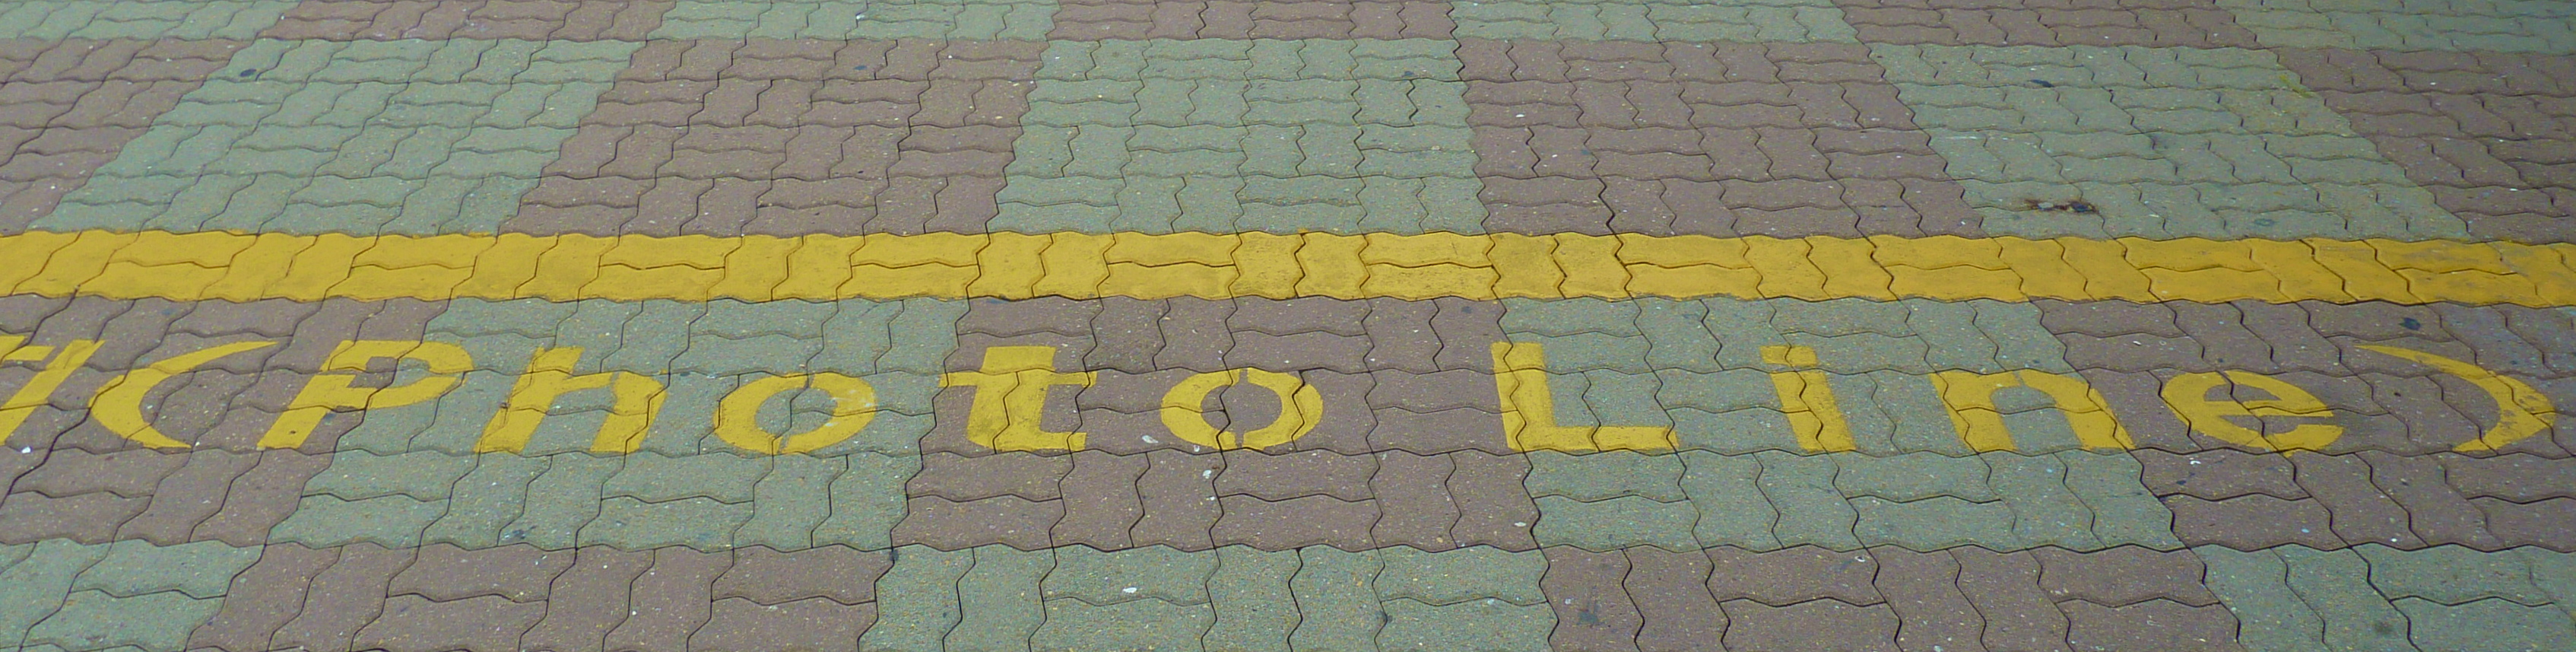
\includegraphics[width=0.7\textwidth]{photos/11/05/p1010331.jpg}}
\end{figure}

The last stop of our DMZ tour was the Dorasan Train station, which is the last SK railroad station before North Korea. For a short period of time, the railroad was used to transport cargo to and from the Kaesong Industrial Region, however, because of <em>"Kim Jong-Il's frikkin mind"</em>, as our tour guide said, the border crossing was shut by NK in 2008. Nowadays, the station serves as a touristic attraction, even though there are few trains coming in every day. For 500KRW you can buy a "ticket" to Pyongyang and go wait on the platform. The train won't come though, so do not spend too much time waiting.

\begin{figure}[h]
\centering\fbox{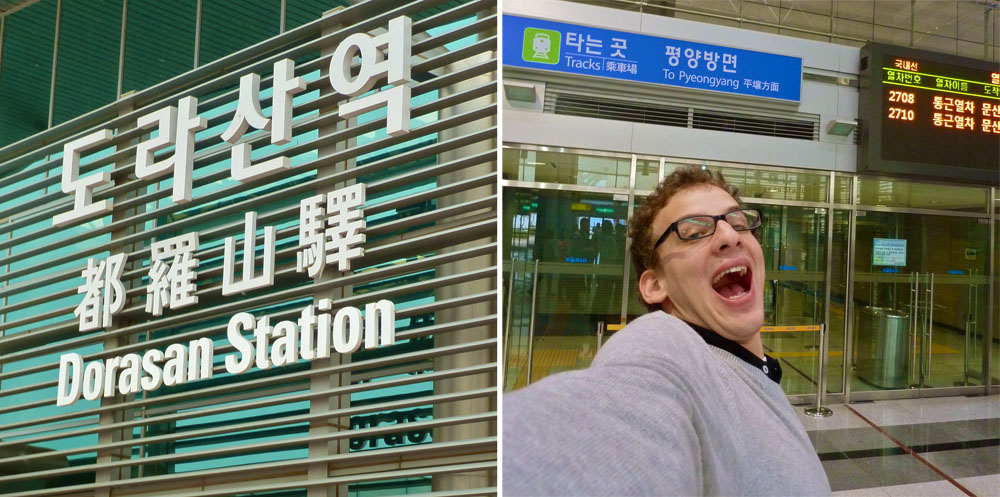
\includegraphics[width=0.6\textwidth]{photos/11/05/combo.jpg}}
\end{figure}

%<p style="text-align:center;"><a href="http://soulexchange.wordpress.com/2011/11/05/between-the-south-and-the-north/combo/" rel="attachment wp-att-299"><img class="size-medium wp-image-299 aligncenter" title="combo" src="http://soulexchange.files.wordpress.com/2011/11/combo.jpg?w=530" alt="" width="530" height="263" /></a></p>

After lunch, which was a very disappointing bulgogi, we moved to a different bus and set off for the second part of our trip, the JSA. Before that, we were warned that the security measures and rules are much stricter than in the DMZ. First thing: No Koreans. For security reasons, Koreans are not allowed to participate in the JSA visit. Secondly, there is a dress code, which prohibits army-like clothes, shorts, flip-flops etc. Thirdly, no communication with North Koreans is allowed. This includes both verbal and non-verbal means, such as waving. Moreover, pointing is prohibited, as it may look like pointing a gun. Lastly, photography is even more restricted than in DMZ.

The JSA is a military facility that lies directly on the Military Demarcation Line. Half of it belongs to South Koreans, that operate it together with U.S. forces, and the second half is North Korean. It is the only place where the two sides directly face each other. It is understandable that the security precautions are so strict. Each bus got it's own armed "guard", that was taking care of our security during the visit. Our guy was a U.S. paratrooper named Muniz. After an ID check we went for a short briefing about the history of JSA, which was a little boring. The interesting part came afterwards. We embarked a military bus and went to visit the Freedom House.

\begin{wrapfigure}{L}{0.52\textwidth}
\vspace{-12pt}
\centering\fbox{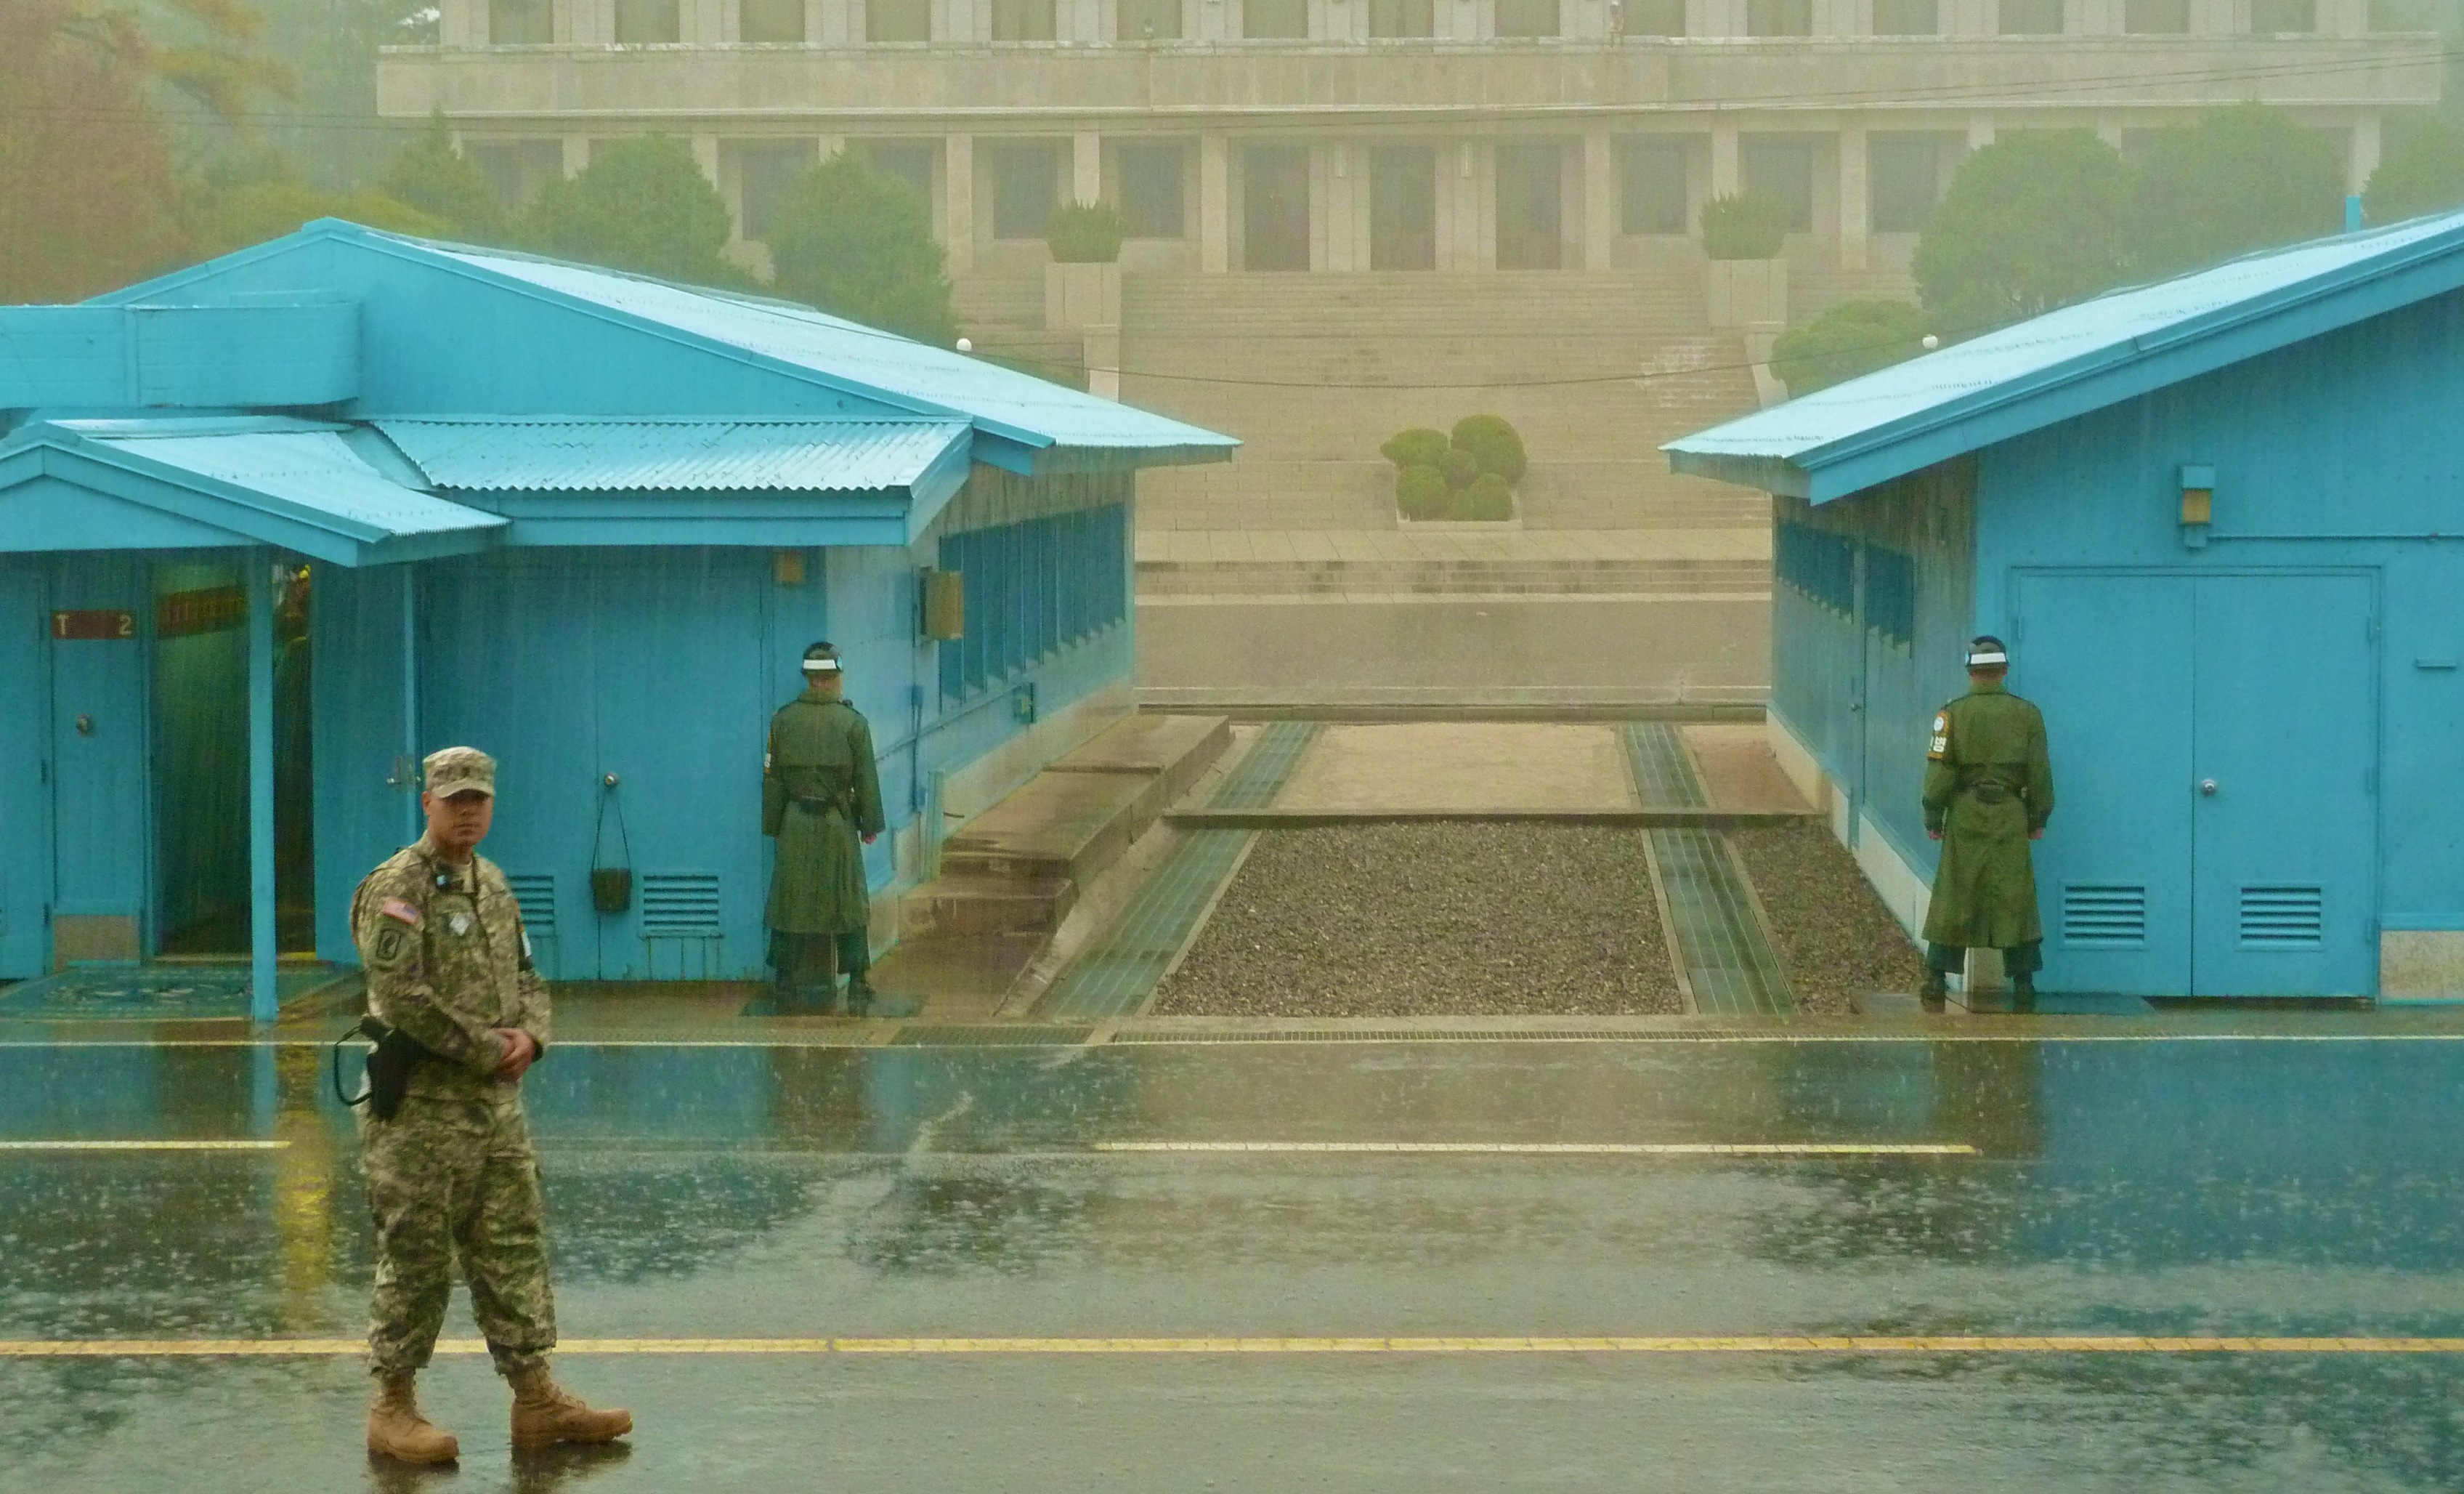
\includegraphics[width=0.52\textwidth]{photos/11/05/p1010377.jpg}}
\vspace{-26pt}
\end{wrapfigure}

%[caption id="attachment_300" align="aligncenter" width="530" caption="The South Korean side of the neutral buildings — The big building in the background is North Korean Panmungak"]<a href="http://soulexchange.wordpress.com/2011/11/05/between-the-south-and-the-north/p1010377/" rel="attachment wp-att-300"><img class="size-medium wp-image-300" title="The South Korean side of the neutral buildings" src="http://soulexchange.files.wordpress.com/2011/11/p1010377.jpg?w=530" alt="The South Korean side of the neutral buildings" width="530" height="353" /></a>[/caption]

Some of you might have seen the JSA before. There are two main buildings — the Freedom House (SK) and Pan\-mun\-gak (NK). Between them is some sort of neutral zone, that is dissected by the Military Demarcation Line. In the center there are several blue buildings that serve as negotiation rooms for the representatives of the two sides. These houses are permanently guarded by elite soldiers and despite the terrible weather, the four SK soldiers were standing there in the rain, partially hidden behind the building, their shades on.

South Korea has pretty strong requirements on the JSA guards. Firstly, they have to be taller than 1,77m. Secondly, they have to have a black belt in either Taekwondo or Judo. The height serves as an intimidation tactics against North Koreans, that are generally smaller. Moreover, SK guards stand in a modified Taekwondo posture, that demonstrates power. They all wear black shades to increase the intimidation factor. Frankly, these guys look really scary, with their angry facial expressions and latent power, that is so apparent despite them standing absolutely still.

When we were waiting outside the negotiation building, there was no NK personnel on guard. However, one guy was standing in front of the Panmungak, observing us through binoculars. It was such a weird feeling, being watched by a North Korean guy, while taking pictures of him. I really wonder what was going through his head at the moment. It was quite a bizarre experience, and it seriously gave me chills — I was standing some 50 meters from North Korea, one of the currently most feared countries, chatting with friends and being all excited about seeing a "real North Korean". Weird.

%<a href="http://soulexchange.wordpress.com/2011/11/05/between-the-south-and-the-north/p1010382/" rel="attachment wp-att-301"><img class="aligncenter size-medium wp-image-301" title="North Korean dude" src="http://soulexchange.files.wordpress.com/2011/11/p1010382.jpg?w=530" alt="North Korean dude" width="530" height="241" /></a>

The grand finale of the JSA visit was the negotiation building, which was at the time guarded by South Koreans, which allowed us to go to the North Korean side, effectively stepping on their territory.

%[caption id="attachment_297" align="aligncenter" width="530" caption="Right now I am standing in North Korea — South Korea is at the left side from the guard, North Korea on the right"]<a href="http://soulexchange.wordpress.com/2011/11/05/between-the-south-and-the-north/p1010393/" rel="attachment wp-att-297"><img class="size-medium wp-image-297" title="Me in North Korea" src="http://soulexchange.files.wordpress.com/2011/11/p1010393.jpg?w=530" alt="" width="530" height="430" /></a>[/caption]

%[caption id="attachment_298" align="aligncenter" width="530" caption="The Demarcation Line as seen from the neutral house"]<a href="http://soulexchange.wordpress.com/2011/11/05/between-the-south-and-the-north/p1010388/" rel="attachment wp-att-298"><img class="size-medium wp-image-298" title="The Demarcation Line" src="http://soulexchange.files.wordpress.com/2011/11/p1010388.jpg?w=530" alt="The Demarcation Line" width="530" height="293" /></a>[/caption]

After that we returned to our bus and went home. I managed to sleep all the way to Seoul, partially reducing my sleeping debt.

\begin{wrapfigure}{R}{0.42\textwidth}
\vspace{-12pt}
\centering\fbox{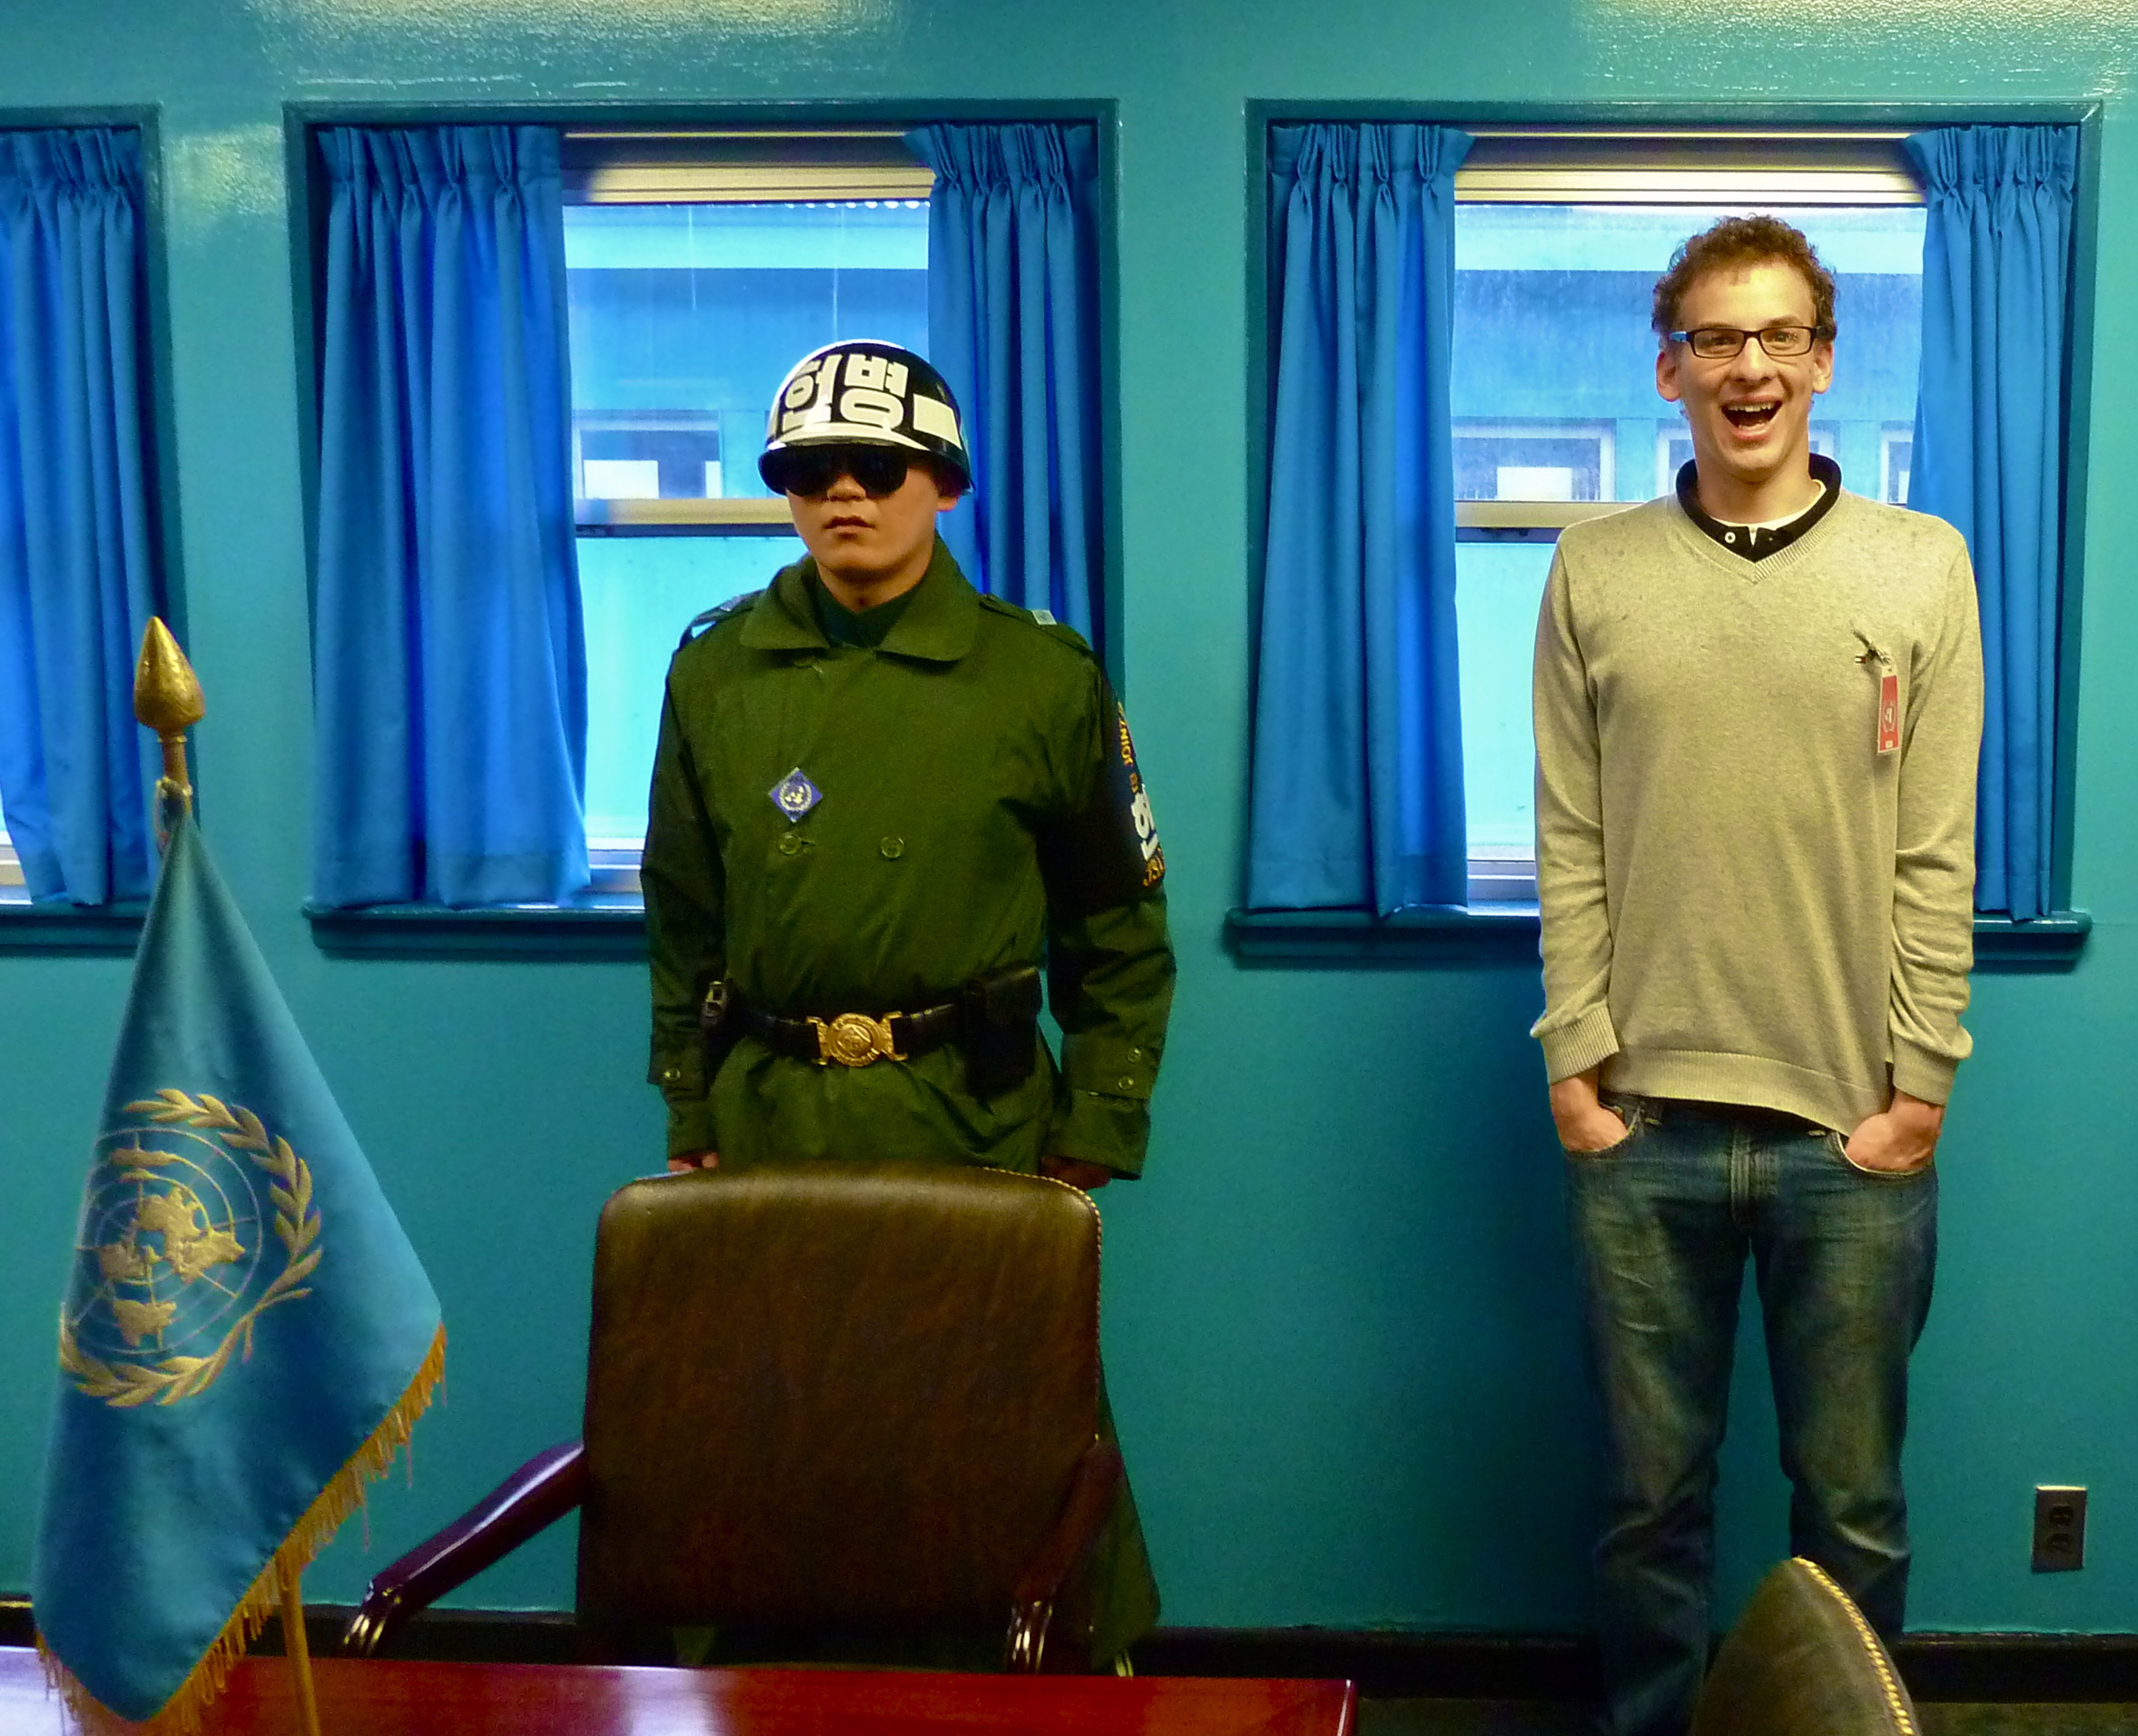
\includegraphics[width=0.42\textwidth]{photos/11/05/p1010393.jpg}}
\vspace{-24pt}
\end{wrapfigure}So, DMZ+JSA, thumbs up or down? I have mixed feelings about that. The first part (DMZ) was not really exciting. Yes, we got to see a bridge and a tunnel, but that is not really connected to the current reality, which devaluates the experience for me. Especially because all the places are "tricked out" for tourists, so it is not even something pure and raw. On the other hand, the JSA was quite amazing. We all felt that there is a latent threat in the air, that probably won't be realized, but you never know. Two armed soldiers in each bus and a jeep with few more in the front showed that everybody takes the situation seriously. After all, I am happy that I went on this trip. It was expensive, I have to admit that, but it was also quite a unique experience. And honestly, who had been to North Korea, huh?
	\end{content}
\end{post}
